\chapter{Parte I}

\section{Generazione delle copie}
In questa prima fase abbiamo generato delle copie degli spettri master in modo tale da poter allenare la rete a riconoscere le differenze tra gli spettri master e copia nella fase succesiva. Affinchè siano rispettati i requisiti, è necessario che gli spettri copia siano solo lievemente differenti dagli originali, di modo che il colore rapresentato dalla copia sia molto simile. Per fare ciò abbiamo preso in considerazione varie tecniche, tra le quali:
\begin{itemize}
	\item sommare un numero random a tutti i campioni dello spettro
	\item moltiplicare tutti i campioni per un numero random
	\item dividere lo spettro in 3 fasce, generare 3 numeri random, sommare il numero random a tutti i campioni della fascia corrispondente
	\item dividere lo spettro in 3 fasce, generare 3 numeri random, moltiplicare il numero random per tutti i campioni della fascia corrispondente
\end{itemize}

Tutti i metodi sono risultati efficaci a patto di regolare oppurtunamente il range di generazione dei coefficienti randomici. L'addizione e la moltiplicazione sono sostanzialmente equivalenti, anche se i coefficienti hanno un diverso peso sul rumore. Per generare le copie abbiamo deciso di utilizzare il rumore moltiplicativo. Abbiamo deciso di utilizzare tutte le alternative allo scopo di avere copie generate in modo variegato.

Per ogni colore del set master generiamo 10 copie, di cui 5 sono disturbate moltiplicando tutti i campioni dello spettro per un numero random piccolo, mentre le restanti 5 sono disturbate su 3 fasce diverse dello spettro. Infine sommiamo un rumore a media nulla molto piccolo a tutti i campioni degli spettri copia. Il codice seguente lo copie dello spettro disturbato \textit{specnoisedP} a partire da \textit{specmasterP}.

\begin{lstlisting}
for i_spec = 1:1269
    for sampl = 1:copies
        specmasterP(:, (i_spec-1)*copies + sampl) = spectra(:, i_spec);

        if( sampl <= floor(copies/2) )
        	a = random('unif',0.95,1.12);
            specnoisedP(:, (i_spec-1)*copies + sampl) = spectra(:,i_spec) * a;
        else
            %DIVIDE BY 3
            a = random('unif',0.97,1.12);
            b = random('unif',0.97,1.12);
            c = random('unif',0.97,1.12);
            specnoisedP(1:146, (i_spec-1)*copies + sampl) = spectra(1:146, i_spec) * a;
            specnoisedP(147:300, (i_spec-1)*copies + sampl) = spectra(147:300, i_spec) * b;
            specnoisedP(301:421, (i_spec-1)*copies + sampl) = spectra(301:421, i_spec) * c;
        end 
        r = -0.0005 + 0.001 * rand(421,1);
        specnoisedP(:, (i_spec-1)*copies + sampl) = specnoisedP(:, (i_spec-1)*copies + sampl) + r;
    end
end
\end{lstlisting}
Forniamo alcuni esempi significativi di coppie di colore generate (originale, copia).

\begin{figure}
\begin{center}
	
\includegraphics[scale=0.5]{images/rete1-colore1.PNG}
	
\includegraphics[scale=0.5]{images/rete1-colore2.PNG}
	
\includegraphics[scale=0.5]{images/rete1-colore3.PNG}
	
\includegraphics[scale=0.5]{images/rete1-colore4.PNG}
\end{center}
\caption{Esempi di copie generate (originale, copia)}
\end{figure}

Dopo una verifica visiva possiamo monitorare di quanto le copie siano state disturbate, in modo aggregato, rispetto al colore master. Per calcolare la differenza tra la copia e master è necessario convertire gli spettri in coordinate L*a*b ed infine calcolare le distanze euclidee. 
\begin{equation}\label{eqn:formula}
        \Delta E^* = \sqrt{(L_1^*-L_2^*)^2+(a_1^*-a_2^*)^2+(b_1^*-b_2^*)^2}
\end{equation}
Per convertire gli spettri in coordinate L*a*b abbiamo usato la funzione \(roo2lab()\) del tool optrop per MATLab ed infine abbiamo calcolato le distanze euclidee tramite la funzione \(de()\) . Possiamo rappresentare la distribuzione delle distanze in un istogramma.

\begin{figure}
\begin{center}
	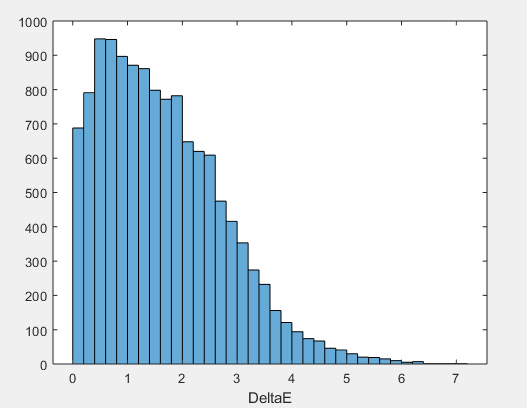
\includegraphics[scale=0.8]{images/rete1-istogramma-deltae.PNG}
\end{center}
\caption{Istogramma delle DeltaE delle coppie (master, copia disturbata)}
\end{figure}

Dal grafico è possibile notare come le coppie stiano nel range 0-4 circa, confermando il fatto che le copie generate siano più o meno simili a quelle originali, come richiesto dalle specifiche.

\section{Feature Selection/Extraction}
Affichè la rete riconosca lo spettro ma sia anche efficiente è necessario che quest'ultimo sia compresso e riassunto da delle features. Ricordiamo infatti, che lo spettro è rappresentato tramite 421 campioni, pertanto vanno selezionate le caratteristiche essenziali in modo da abbattere gli ingressi da fornire alla rete.

A questo punto dobbiamo scegliere quale feature estrarre. Abbiamo ragionato principalmente sul materiale fornito dalle specifiche, in particolare su come viene calcolato il colore percepito dall'occhio umano secondo gli standard CIE. Sono state prese in considerazione diverse funzioni, cioè \textit{mean, mode, median, var, skewness, min and max (sia massimi/minimi che punti di massimo/minimo)}. La \textit{feature selection} è stata effettuata dividendo lo spettro in 6 parti uguali e applicando, per ognuna di queste, le funzioni prima elencate. Pertanto ogni funzione fornisce 6 features rappresentative dello spettro considerato.

Il metodo utilizzato per la \textit{feature extraction} è quello fornito da MATLab attraverso la funzione \textit{sequentialfs()}. Il numero di feature estratte è stato oggetto di analisi al fine di individuare il minor numero di feature, in modo tale da rendere la rete efficiente, e ottenere le migliori prestazioni in termine di errore quadratico medio. Dopo attente analisi abbiamo deciso di selezionare 12 features visto che queste risultano sufficienti per ottenere un errore quadratico medio pari a 0.01.

\section{Risultati}
La rete che ha i risultati migliori è quella con 12 neuroni nello strato di ingresso e 8 nell'hidden layer (unico strato). Abbiamo eseguito la prova per 10 ripetizioni ed abbiamo ottenuto un \textit{Mean Squared Error} pari a circa 0.017 e un valore \textit{R (Regression)} pari a \(0.99338 \pm 0.0004\).

\begin{figure}[!ht]
\begin{center}
	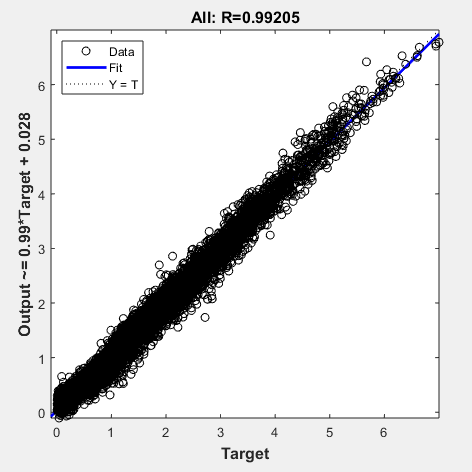
\includegraphics[scale=0.7]{images/rete1-regression.jpg}
\end{center}
\caption{Retta di Regressione della rete neurale}
\end{figure}

\paragraph{Feature estratte}
Le feature estratte dalla \textit{sequentialfs} sono state le seguenti:
\\\\
\textbf{master}: mean(2), mode(3), median(4), median(5), skewness(3), maxYValue(2), minYValue(1)
\\
\textbf{copie}: mean(2), var(2), mode(1), skewness(3), maxYValue(2)
\\\\(1,2,3) indicano i 3 range dello spettro equidimensionati sulla quale le funzioni sono applicate
\\(4,5) sono 2 range aggiuntivi, che si sovrappongono ai precedenti (dividono lo spettro in 2)

Tuttavia differenti esecuzioni hanno portato, spesso, all'estrazione di feature differenti: questo può essere dovuto alla correlazione tra le varie funzioni scelte (es. la skewness è calcolata dal mean e dalla varianza).